% sec4a.tex —— 块 c04｜原文 p20–p25｜§4.1–§4.2
% 公式号 (39)–(50)；编号环境 4.1–4.13。
% 块止于 Corollary 4.13 的陈述；其证明（含式 (51)）、Remark 4.14 与式 (52) 均在 p26，归 c05。

% [原文 p.20]
确定 2 维超对称量子场论的完整数学内容，仍是一个未解问题。大致轮廓来自超对称量子力学的环路空间推广，如 Witten 所述 [Wit88a]，并在 §4.1–4.2 中综述。然而从一开始人们就知道，这一过于简单的推广无法捕捉 2 维超对称场论的附加数据与性质，例如状态空间上的实结构 [Wit87] 以及反常相消数据 [Wit88a, §3]。这些由物理考量所预期的数据，在 Stolz 与 Teichner 的配边框架 [ST11] 中自然地出现——且出于纯几何的理由。我们在 §4.3–4.4 中解释其中的若干方面。在 §4.5 中，我们勾勒全扩张超对称场论的预期特征，并对通向猜想 1.1 的若干可能途径作些推测。

\subsection{2 维超对称量子场论的基本数据}

作为一阶近似，2 维量子场论是量子力学的环路空间版本 [Wit88a]：除状态空间与哈密顿量之外，还有作用在状态上的 $S^1_r$-作用，其中 $S^1_r=\R/2\pi r\Z$ 是半径为 $r$ 的圆周。无穷小的 $S^1_r$-作用定义动量算子 $P^{(r)}\in\mathrm{End}(\cH)$，其谱落在 $\frac1r+\frac{n}{24r}\cdot\Z\subset\R$ 中。\footnote{对 $n\in\Z$，$n/24$ 的平移编码了理论的\emph{次数}，它与下文所述的反常有关。} 对每个 $r\in\R_{>0}$，哈密顿量 $H^{(r)}$ 与动量算子 $P^{(r)}$ 定义一个半群表示（semigroup representation）
\begin{equation}
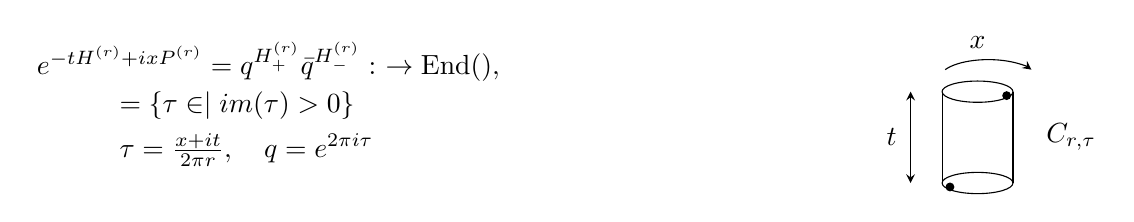
\begin{tikzpicture}[baseline=(current bounding box.center), >=stealth]
  \node[anchor=west] (a) at (0,0.62) {$e^{-tH^{(r)}+ixP^{(r)}}=q^{H^{(r)}_+}\bar q^{H^{(r)}_-}:\ \HH\to\mathrm{End}(\cH),$};
  \node[anchor=west] (b) at (1.05,0.06) {$\HH=\{\tau\in\C\mid\operatorname{im}(\tau)>0\}$};
  \node[anchor=west] (c) at (1.05,-0.50) {$\tau=\frac{x+it}{2\pi r},\quad q=e^{2\pi i\tau}$};
  \draw (11.62,-0.92) -- (11.62,0.24);
  \draw (12.52,-0.92) -- (12.52,0.24);
  \draw (12.07,0.24) ellipse (0.45 and 0.135);
  \draw (12.07,-0.92) ellipse (0.45 and 0.135);
  \fill (12.44,0.19) circle (1.6pt);
  \fill (11.72,-0.97) circle (1.6pt);
  \draw[<->] (11.22,-0.92) -- (11.22,0.24);
  \node at (10.98,-0.34) {$t$};
  \draw[->] (11.66,0.52) arc (152:28:0.62 and 0.24);
  \node at (12.07,0.86) {$x$};
  \node[anchor=west] at (12.82,-0.34) {$C_{r,\tau}$};
\end{tikzpicture}
\tag{39}
\end{equation}
它推广了量子力学中的时间演化半群 (6)，其中（为后文方便）引入算子 [Wit86, Eq. 106]
\begin{equation}
H^{(r)}_+=\frac r2\left(H^{(r)}+P^{(r)}\right),\qquad H^{(r)}_-=\frac r2\left(H^{(r)}-P^{(r)}\right).
\tag{40}
\end{equation}

% [Tutor Note: (39) 右侧的圆柱示意（高 $t$、旋转 $x$、两个标记点、标签 $C_{r,\tau}$）用内联 TikZ 重绘，它是公式的一部分而非编号图，故不用 \figomit；原图的两点标出粘合时两个边界点的对应。]
% [Tutor Note: 谱的关系可验证：由 (40) 得 $H^{(r)}_++H^{(r)}_-=rH^{(r)}$、$H^{(r)}_+-H^{(r)}_-=rP^{(r)}$，故 $rP^{(r)}$ 的谱为 $\Z+\frac n{24}$、$H^{(r)}_\pm$ 的谱为 $\frac12\left(\lambda\pm(k+\frac n{24})\right)$，这正是 (50) 与图 6 两条轴标注的来源。]
% [Tutor Note: $n$ 在此首现而未加说明（到例 4.3 才明确 $n=\dim M$）；原文即如此，读者可先把它读作理论的次数。]

正如 (39) 右方所示，可以把这一半群表示几何地重新表述：参数 $(r,\tau)$ 确定一个圆柱 $C_{r,\tau}$，它被看作半径为 $r$ 的圆周之间的一条欧几里得（即平坦 Riemann）配边，其中复参数 $\tau$ 编码圆柱之高 $t$，以及度量两个边界圆周参数化之差的旋转 $x\bmod 2\pi r$ [Wit86, Figure 2]。\emph{配分函数}是半群表示 (39) 的特征（character，即迹），
\[
Z(r,\tau):=\Tr\left(q^{H^{(r)}_+}\bar q^{H^{(r)}_-}\right)\in C^\infty(\R_{>0}\times\HH),\qquad r\in\R_{>0},\ \tau\in\HH.
\]

路径积分论证 [Wit86, §3] 把 $Z(r,\tau)$ 与理论在环面上的取值等同起来，该环面为 $T_{r,\tau}=\R^2/(2\pi r\Z\oplus 2\pi\tau\Z)$，由把圆柱两端粘合而成。一般的不变性使人期待这一取值只依赖于底层的% [原文 p.21]
环面，而不依赖于由 $r$ 与 $\tau$ 生成的带基格。群 $\mathrm{SL}_2(\Z)$ 通过改变此格的基而作用，
\[
\begin{bmatrix} a & b\\ c & d \end{bmatrix}\cdot(r,\tau)=\left(r|c\tau+d|,\ \frac{a\tau+b}{c\tau+d}\right),\qquad \begin{bmatrix} a & b\\ c & d \end{bmatrix}\in\mathrm{SL}_2(\Z)
\]
于是朴素地，人们可能期待 $Z(r,\tau)$ 是 $\mathrm{SL}_2(\Z)$-不变的函数。然而，追踪 $P^{(r)}$ 的谱中 $n/24r$ 的平移，可见 $Z(r,\tau)$ 只在一个由特征标 $\chi^n\colon\MP_2(\Z)\to\C^\times$ 编码的单位根的意义下不变 [Wit87]
\begin{equation}
Z(r,\tau)\in C^\infty(\R_{>0}\times\HH;\chi^n)^{\MP_2(\Z)}
\tag{41}
\end{equation}
其中 $\MP_2(\Z)\to\mathrm{SL}_2(\Z)$ 是 metaplectic 二重覆盖。$Z(r,\tau)$ 不能 $\mathrm{SL}_2(\Z)$-不变，这是反常理论的一个标志 [Fre87, §4]。事实上，$Z(r,\tau)$ 决定了欧几里得环面上 Pfaffian 线丛的第 $n$ 次张量幂的一个截面，而该线丛的截面与权 $n/2$ 的模形式密切相关；见注 4.1。

% [Tutor Note: (41) 记号的读法：$C^\infty(\R_{>0}\times\HH;\chi^n)$ 是取值于线丛 $\chi^n$ 的截面空间，上标 $\MP_2(\Z)$ 取 $\MP_2(\Z)$-不变部分；$\chi^n$ 即 (45) 中特征标 $\chi$ 的 $n$ 次幂（$n$ 次张量幂 $\leftrightarrow$ 权 $n/2$），与 (49) 一致。]

接下来加入超对称：\footnote{本讨论只考虑 Ramond 扇区；在 §4.3 中我们会纳入 Neveu--Schwarz 扇区。} $H^{(r)}_+$ 的 $\mathcal N_+$ 个奇的交换平方根、与 $H^{(r)}_-$ 的 $\mathcal N_-$ 个奇的交换平方根，这些数据称为 $\mathcal N=(\mathcal N_+,\mathcal N_-)$ \emph{超对称}。 我们将关注 $\mathcal N=(0,1)$ 超对称，即单个奇算子 $Q^{(r)}$，满足
\begin{equation}
(Q^{(r)})^2=\frac12[Q^{(r)},Q^{(r)}]=H^{(r)}_-,\qquad [Q^{(r)},P^{(r)}]=[Q^{(r)},H^{(r)}]=0.
\tag{42}
\end{equation}

推广超对称量子力学中的时间演化 (26)，算子 $Q^{(r)}$ 把半群表示 (39) 提升为一个\emph{超半群}（supersemigroup）表示
\begin{equation}
q^{H^{(r)}_+}\bar q^{H^{(r)}_-+\sqrt{2\pi i}\,\theta Q^{(r)}},\qquad \mathbb H^{2|1}\to\mathrm{End}(\cH)
\tag{43}
\end{equation}
其中 $\HH^{2|1}\subset\R^{2|1}$ 是超 Lie 群 $\R^{2|1}$ 的上半空间，其乘法为
\begin{equation}
(\tau',\bar\tau',\theta')\cdot(\tau,\bar\tau,\theta)=(\tau'+\tau,\ \bar\tau'+\bar\tau+\theta'\theta,\ \theta'+\theta),\qquad (\tau',\bar\tau',\theta'),(\tau,\bar\tau,\theta)\in\R^{2|1}.
\tag{44}
\end{equation}
这一超半群表示同样可以几何地解释，但此时是作为某个\emph{超圆柱}（super cylinder）范畴的表示，其几何参数为 $(r,\tau,\bar\tau,\theta)\in\R_{>0}\times\HH^{2|1}$。类似地，该半群表示的迹对应理论在\emph{超环面}（super torus）上的取值，这施加一个与 (41) 类似的预期不变性。这一几何示意地画在图 5 中。

% [Tutor Note: $\sqrt{2\pi i}$ 在原文里只覆盖 $2\pi i$，$\theta Q^{(r)}$ 在根号之外；这是超半群上 $q^{H_+}\bar q^{H_-+(\text{odd})}$ 的标准写法，不要误读成 $\sqrt{2\pi i\,\theta Q^{(r)}}$。]
% [Tutor Note: 原文第 9 号脚注（本译本第 2 号脚注）只考虑 Ramond 扇区；Neveu--Schwarz 扇区要到 §4.3（c05 块）才纳入，故本块的 $\mathcal N$ 只指 Ramond 侧。]

% [原文 p.21]
\figomit{5}{半群中的复合对应圆柱的粘合，而环面上的取值对应迹。}

\begin{remark}[4.1]
考虑分类带奇 spin 结构的 spin 椭圆曲线的商叠 $\HH/\!/\MP_2(\Z)$，其中 $\MP_2(\Z)$ 经二重覆盖 $\MP_2(\Z)\to\mathrm{SL}_2(\Z)$ 以分式线性变换作用在 $\HH$ 上。该叠上有一个线丛，它由如下特征标确定：
\begin{equation}
\chi\colon\MP_2(\Z)\to\MP_2(\Z)/[\MP_2(\Z),\MP_2(\Z)]\simeq\Z/24\hookrightarrow\C^\times
\tag{45}
\end{equation}
\end{remark}

% [Tutor Note: 原文注 4.1 在式 (45) 处收尾，p22 另起一段、用正体 "which is the Pfaffian line bundle…" 接着把这句话说完；中译为免段落以关系从句开头，在 p22 段首改写为「这一线丛就是……」，语义未变。]
% [Tutor Note: 记号 $\HH/\!/\MP_2(\Z)$ 表示作用群胚的商（作用非自由之处保留稳定化子），与轨道空间 $\HH/\MP_2(\Z)$ 不同；该商是分类 spin 椭圆曲线的模叠。]

% [原文 p.22]
这一线丛就是 Pfaffian 线丛 $\mathrm{Pf}\to\HH/\!/\MP_2(\Z)$ [Fre87, §4]。另一个线丛的截面是权 $1/2$ 的模形式，即满足
\begin{equation}
f\left(\frac{a\tau+b}{c\tau+d}\right)=\sqrt{c\tau+d}\,f(\tau).
\tag{46}
\end{equation}
的全纯函数 $f(\tau)$。

由 (46) 确定的线丛与 Pfaffian 线丛都是 Picard 群 $\mathrm{Pic}(\HH/\!/\MP_2(\Z))\simeq\Z/24$ 的生成元，因而彼此同构。Dedekind $\eta$ 函数给出一个显式同构，特别地给出整体截面上的一个双射
\[
\Gamma(\HH/\!/\MP_2(\Z);\mathrm{Pf}^{\otimes n})\xrightarrow{\ \sim\ }\mathrm{MF}_{n/2},\qquad Z(q)\mapsto\eta(q)^n Z(q),\qquad \eta(q)=q^{1/24}\prod_{k>0}(1-q^k)
\]
这可以由 $\eta(q)$ 的标准变换性质验证。模形式与 $\HH$ 上在 $\MP_2(\Z)$ 作用下带相位变换的函数之间的这一双射，在物理文献中被广泛使用，例如 [Wit88a, Eq. 18]。

% [Tutor Note: (46) 中 $\sqrt{c\tau+d}$ 的符号取定属于 $\MP_2(\Z)$ 的额外数据（二重覆盖），单看 $\mathrm{SL}_2(\Z)$-不变性无法定出；核验方式：对 $\gamma$ 与 $-\gamma$ 取同一 $\tau$，$f$ 的值相差一个符号。]
% [Tutor Note: 上式 $\mathrm{MF}_{n/2}$ 指权 $n/2$ 的模形式空间（此处不取整模形式）；与后文 $\mathrm{MF}^{\Z}$（整模形式）区别开。乘法因子 $\eta(q)^n$ 恰是权 $n/2$ 的，故双射把带相位的函数送到真模形式。]

\begin{example}[4.2（手征理论）]
数据 (40) 在 $H^{(r)}_-=0$ 时确定一个\emph{手征}场论。\footnote{chiral 的更常见用法假定 $H^{(r)}_+=L_0$ 与 $H^{(r)}_-=\bar L_0$ 是共形场论数据的一部分，其 Virasoro 生成元为 $L_k$，且 $k\in\Z$ 时 $\bar L_k=0$。} 手征理论有一个典范的超对称扩张，即取 $Q^{(r)}=0$；于是（沿用例 3.11）手征理论是拓扑理论在 2 维的相关推广，进一步讨论见式 (56)。就目前而言，我们指出：任何手征共形场论（例如顶点算子代数的数据）都给出一个 2 维手征理论，从而给出一个超对称理论。
\end{example}

% [Tutor Note: 原文第 10 号脚注（本译本第 3 号脚注）末尾作「$\bar L_k=0$ for $k\in\Z$」，字面读则右移 Virasoro 模全为零、与 $H^{(r)}_-=\bar L_0$ 相容但过于强；常见约定是 $k>0$ 时 $\bar L_k=0$。照排不改，存疑已在回报中列出。]
% [Tutor Note: 例 4.2 说手征 $\Leftrightarrow H^{(r)}_-=0$，而由 (42) 有 $H^{(r)}_-=(Q^{(r)})^2$，故 $Q^{(r)}=0$ 是唯一可能的超对称扩张（奇数算子平方为 $0$ 强于为零）；这正是本例"典范扩张"的含义。]

\begin{example}[4.3（超对称 $\sigma$ 模型与 Witten 亏格）]
设 $M$ 是 Riemann 的 spin 流形。Witten 在 $LM$ 上的旋量丛沿 $M\hookrightarrow LM$ 的限制（按定义）是向量丛的形式幂级数 [Wit88a, Eq. 24]
\begin{equation}
\cS\otimes\left(\bigotimes_{m\ge1}\mathrm{Sym}_{q^m}(TM)\right)=\cS+q\cS\otimes TM+q^2\cS\otimes\left(TM+\mathrm{Sym}^2(TM)\right)+\cdots
\tag{47}
\end{equation}
其中 $\cS$ 是 $M$ 上的旋量丛，而 $\mathrm{Sym}_q(TM)=1+qTM+q^2\mathrm{Sym}^2(TM)+\cdots$。以 $W_k(TM)$ 记 (47) 中 $q^k$ 的系数，以 $\cH$ 记 (47) 的截面的 Hilbert 完备化。对每个 $r\in\R_{>0}$，通过
\[
Q^{(r)}|_{W_k(TM)}=D\!\!\!/\otimes W_k(TM)+\sqrt{k}/\sqrt{r},\qquad P^{(r)}|_{W_k(TM)}=k/r-n/24r,\qquad n=\dim(M)
\]
在 $\cH$ 上定义算子 $P^{(r)}$ 与 $Q^{(r)}$，其中 $D\!\!\!/$ 是 $M$ 上 $\mathrm{Cl}_{-n}$-线性的 Dirac 算子。这给出一个超对称场论的输入数据 (42)。Atiyah--Singer 指标定理计算相应半群表示的（Clifford）超迹（见注 4.4）
\begin{equation}
Z(r,\tau)=\Tr_{\mathrm{Cl}_{-n}}\left(q^{H^{(r)}_+}\bar q^{H^{(r)}_-}\right)=q^{-n/24}\sum_{k=0}^{\infty}q^k\hat A(M,W_n(TM))
\tag{48}
\end{equation}
其中 $\hat A(M,W_n(TM))$ 是扭 $\hat A$ 类（twisted $\hat A$-class）。Zagier [Zag86] 验证了：当第 1 有理 Pontryagin 类 $p_1(TM)\in H^4(M;\Q)$ 为零时，归一化配分函数 $\eta(q)^n q^{-n/24}\sum_{k=0}^\infty q^k\hat A(M,W_n(TM))$ 为权 $n/2$ 的模形式。注 4.1 随即确认：$\MP_2(\Z)$ 在 $Z(r,\tau)$ 上的作用通过一个 24 次单位根给出。
\end{example}

% [Tutor Note: **原文笔误**：(48) 及其后一句都写 $\hat A(M,W_n(TM))$，但 $W_n$ 与求和指标 $k$ 无关，级数会塌成几何级数、不可能是权 $n/2$ 的模形式；按上文对 $W_k(TM)$（即 $q^k$ 的系数）的定义，此处应为 $\hat A(M,W_k(TM))$。已照排原文，并在回报中登记 ERRATA。]
% [Tutor Note: $\mathrm{Cl}_{-n}$ 指 $\R^n$ 上由负定二次形式给出的 Clifford 代数（它线性地作用在旋量丛 $\cS$ 上），与 $\mathrm{Cl}_n$ 差一个整体符号；原文排版把 Cl 印成空心体 $\mathbb Cl$，中译统一作 $\mathrm{Cl}$。]

\begin{remark}[4.4]
Clifford 模 $V$ 上 $\mathrm{Cl}_n$-线性自同态 $T$ 的\emph{Clifford 超迹}定义为 [ST04, Definition 3.2.16]
\[
\mathrm{sTr}_{\mathrm{Cl}_n}(T)=\mathrm{sTr}(\Gamma_n\circ T),\qquad T\colon V\to V
\]
其中 $\Gamma_n=(2i)^{-n/2}e_1\cdots e_n\in\mathrm{Cl}_n$，而 $\{e_1,\dots,e_n\}$ 是 $\R^n$ 的标准基，它在包含 $\R^n\subset\mathrm{Cl}_n$ 下与 Clifford 代数的（奇）元素等同。
\end{remark}

% [Tutor Note: 这里的 sTr 是通常的超迹（偶/奇部分取迹后相减），$\Gamma_n$ 用于把 Clifford 模上的迹化成普通超迹；核验：$n$ 为偶数时 $\Gamma_n$ 与 $\mathrm{Cl}_n$ 的偶部交换，故 sTr 对 Clifford 线性的 $T$ 有定义。]

% [原文 p.23]
\figomit{6}{$\qft^n$ 中的一个对象确定一个从 $\R_{\ge0}$ 到 $\R^2$ 中构形的连续映射，其标号是子空间 $\cH(k)_\lambda\subset\cH_n$，由 $k\in\Z$ 与 $\lambda\in\R$ 编号，其中 $P^{(r)}$ 与 $H^{(r)}$ 共享一个特征子空间，特征值分别为 $k/r+n/24$ 与 $\lambda$。把这些特征子空间排在平面中是方便的：横轴为 $rP^{(r)}$ 的特征值，纵轴为 $H^{(r)}_-$ 的特征值（即能量与动量之差）。超对称随即要求纵向的特征值非负，并给每个标号配上一个由 $Q^{(r)}$ 限制到 $\cH(k)_\lambda$ 得到的奇算子。这样对每个 $k\in\Z$ 都得到图 3 的一个副本。}

\begin{remark}[4.5]
有若干正在进行的工作，试图用分析工具严格构造环路空间上的旋量丛及其伴随的 Dirac 算子，使得限制到常值环路时回到例 4.3，例如见 [ST05, KM13, KM15, KLW22, LW23, Lud23]。更代数的方法则在常值环路的形式邻域中构造了密切相关的对象，例如 [GMS00, GMS04, Cos10, Cos11]。
\end{remark}

\subsection{2 维场论的逼近范畴}

下面我们给出 2 维量子场论的一些初步（且不完整的）定义，它们汇集了上述算子 (40) 与 (42) 的数据与性质。鉴于例 4.3，我们在下面的定义中加入 Clifford 次数：对每个 $n\in\Z$ 固定一个分次 $\mathrm{Cl}_n$-模 $\cH_n$，例如对无穷维可分 Hilbert 空间 $\cH$，取 $\cH_n=\mathrm{Cl}_n\otimes\cH$。

\begin{definition}[4.6]
定义拓扑群胚 $\qft^n$：其对象是 $\cH_n$ 上满足下述条件的、$\mathrm{Cl}_n$-线性无界偶算子的连续 $\R_{>0}$-族 $\{H^{(r)}_+,H^{(r)}_-\}_{r\in\R_{>0}}$：
\begin{enumerate}[label=(\roman*)]
  \item $H^{(r)}_+$ 与 $H^{(r)}_-$ 确定自伴迹类半群表示 (39)；
  \item Clifford 超迹
  \begin{equation}
  \begin{aligned}
  Z(r,\tau)&:=\mathrm{sTr}_{\mathrm{Cl}_n}\left(q^{H^{(r)}_+}\bar q^{H^{(r)}_-}\right),\qquad Z\left(r|c\tau+d|,\frac{a\tau+b}{c\tau+d}\right)=\chi^n(\gamma)Z(r,\tau),\\[2pt]
  \gamma&=\left(\begin{bmatrix}a&b\\c&d\end{bmatrix},(c\tau+d)^{1/2}\right)\in\MP_2(\Z)
  \end{aligned}
  \tag{49}
  \end{equation}
  在由特征标 $\chi^n$（来自 (45)）指定的相位意义下是 $\MP_2(\Z)$-不变的。
\end{enumerate}
$\qft^n$ 中的态射是连续映射 $\R_{>0}\to\mathrm{PU}^\pm(\cH_n)$，它们通过共轭作用在 $H^{(r)}_\pm$ 上。
\end{definition}

% [Tutor Note: (49) 只占一个号，第二行的 $\gamma$ 是给第一行右半式用的；$\gamma$ 就是 $\MP_2(\Z)$ 的元素——二阶矩阵加半整数权因子 $(c\tau+d)^{1/2}$，这正是 $\MP_2$ 作为 $\mathrm{SL}_2(\Z)$ 二重覆盖的体现，不可漏掉。]
% [Tutor Note: 定义 4.6 (ii) 只要求 (49) 在相位 $\chi^n(\gamma)$ 下不变，而不要求严格的 $\MP_2(\Z)$-不变性；这一点在定理 4.11 的证明里被用来推出"权 $-n/2$"而非"权 $0$"。]

算子 $rP=H^{(r)}_++H^{(r)}_-$ 的谱落在离散集 $\Z+\frac{n}{24}$ 中，因此这一谱不依赖于连续参数 $r$。在同构意义下，这给出状态空间的一个分解
\begin{equation}
\cH_n\simeq\bigoplus_{k\in\Z}\cH(k),\qquad H^{(r)}_-(k):=H^{(r)}_-|_{\cH(k)}
\tag{50}
\end{equation}
使 $rP^{(r)}$ 在 $\cH(k)$ 上以 $k+\frac{n}{24}\in\Z$ 作用，而 (50) 中的 $H^{(r)}_-(k)$ 由限制定义。这样一来，$\qft^n$ 中的一个对象可以看作无穷多个量子力学% [原文 p.24]
系统的汇集，其哈密顿量为 $H^{(r)}_-(k)$，对每个动量数 $k\in\Z$ 与半径 $r\in\R_{>0}$ 各一个，其中对半径参数的依赖是连续的。\footnote{更确切地说，$H^{(r)}_-(k)$ 是哈密顿量与相应量子力学系统的一个射影 $S^1$-对称的生成元的组合，见 [Wit99, §1.3]。} 这一直观可以通过图 6 中所示算子 $H^{(r)}_+$ 与 $H^{(r)}_-$ 的构形空间描述精确化：每条竖线是一个构形，它定义一个量子力学系统，另见 [Che08, Figure 4]。

% [Tutor Note: **原文笔误**：此处作 $rP=H^{(r)}_++H^{(r)}_-$，但由 (40) 有 $H^{(r)}_++H^{(r)}_-=rH^{(r)}$、$H^{(r)}_+-H^{(r)}_-=rP^{(r)}$，故应为减号；又 $H^{(r)}_\pm$ 的谱非负（超对称要求纵向特征值非负），若取加号则谱不可能落在 $\Z+\frac n{24}$ 的离散集上。已照排原文并登记 ERRATA。]
% [Tutor Note: (50) 的分解是由 $rP^{(r)}$ 的谱离散且与 $r$ 无关、加上迹类条件得到的（原文归入"如此断言"，未给证明）；注意 $\cH(k)$ 是 $H^{(r)}_-$ 的稳定子空间，故 $H^{(r)}_-(k)$ 有意义。]

\begin{proposition}[4.7]
对每个 $n\in\Z$，存在同伦等价 $|\qft^n|\simeq\BPU^\pm(\cH_n)$。
\end{proposition}

\begin{proof}[略证]
如上所述，对每个权空间 $\cH(k)\subset\cH_n$ 我们得到哈密顿量的连续 $\R_{>0}$-族 $H^{(k)}(r)$。对每个这样的哈密顿量 $H^{(r)}_k$，存在一个把全部特征子空间送到无穷远的形变。这确定一条到基点的收缩同伦，其定义域为 $\{0\}\subset\cH_n$。对每个 $k\in\Z$ 同时施加这些同伦，$\qft^n$ 的对象空间便形变收缩到对应于图 6 中空构形的零理论。由与命题 2.7 相同的论证，得到所说的同伦型。
\end{proof}

% [Tutor Note: 略证中 $H^{(k)}(r)$ 与紧随的 $H^{(r)}_k$ 指同一族哈密顿量，原文两处写法不一致（一处下标为 $k$、一处上标为 $(r)$），照排不改；读时按"固定 $k$、随 $r$ 变化"理解即可。]

\begin{remark}[4.8]
空间 $\BPU^\pm(\cH_n)$ 有一对非平凡同伦群：$\pi_1\BPU^\pm(\cH_n)\simeq\Z/2$，以及 $\pi_3\BPU^\pm(\cH_n)\simeq\Z$。二者由一个非平凡的 $k$-不变量相连。
\end{remark}

与量子力学的情形一样，若加入超对称，$\qft^n$ 的同伦型会变得更有趣。

% [Tutor Note: $\BPU^\pm(\cH_n)$ 是射影酉群的两个连通分支（对应 $\mathrm{PU}$ 的 $\pm$，即行列式相位 $\pm1$）的分类空间；故 $\pi_1=\Z/2$ 来自这两个分支，而非 $\mathrm{PU}(\cH)$ 自身的拓扑。]

\begin{definition}[4.9]
定义拓扑群胚 $\sqft^n$：其对象是 $\mathrm{Cl}_n$-线性无界算子的连续 $\R_{>0}$-族 $\{H^{(r)}_+,Q^{(r)}\}_{r\in\R_{>0}}$，其中 $H^{(r)}_+$ 是偶的、$Q^{(r)}$ 是奇的。这些数据满足两条性质。
\begin{enumerate}[label=(\roman*)]
  \item $H^{(r)}_+$ 与 $Q^{(r)}$ 确定自伴迹类超半群表示 (43)。
  \item 令 $H^{(r)}_-=(Q^{(r)})^2$，则 Clifford 超迹 (49) 在由特征标 $\chi^n$（来自 (45)）指定的相位意义下是 $\MP_2(\Z)$-不变的。
\end{enumerate}
$\sqft^n$ 中的态射是连续映射 $\R_{>0}\to\mathrm{PU}^\pm(\cH_n)$，它们通过共轭作用在 $H^{(r)}_+$ 与 $Q^{(r)}$ 上。
\end{definition}

仿照定义 4.6 之后的讨论，$\sqft^n$ 中的一个对象可以看作无穷多个超对称量子力学系统的汇集，其超对称生成元为 $Q^{(r)}(k):=Q^{(r)}|_{\cH(k)}$，对每个动量数 $k\in\Z$ 与半径 $r\in\R_{>0}$ 各一个。关于构形空间的视角，我们仍参见图 6。

% [Tutor Note: 定义 4.9 里 $H^{(r)}_-$ 不再是独立数据，而是由 (ii) 取成 $(Q^{(r)})^2$；这与定义 4.6 中 $H^{(r)}_\pm$ 并列的写法不同，后者是 4.6 的子情形（$Q=0$ 即得 4.6）。]

\begin{theorem}[4.10（{[ST04, Theorem 1.0.2]} 与 {[Che08, Theorem 2.2.2]}）]
$\sqft^n$ 中对象构成的空间映入 $K_n((q))$，即表示 Tate 曲线上椭圆上同调的谱中的第 $n$ 个空间。
\end{theorem}

\begin{proof}[略证]
把 $\cH\simeq\bigoplus_{k\in\Z}\cH(k)$ 分解为 $rP^{(r)}$ 的权空间，我们得到一个奇的、$\mathrm{Cl}_n$-线性算子的 $\R_{>0}$-族 $\{Q^{(r)}(k)\}_{k\in\Z}$。对每个 $k$ 取固定半径（例如 $r=1$），这确定一个映入定理 3.10 中表示 $K_n$ 的空间的映射。半群上的迹类条件要求 $Q^{(r)}(k)$ 对充分负的 $k$ 表示零类，于是合起来得到一个映入空间 $K_n((q))$ 的映射。
\end{proof}

\begin{theorem}[4.11（{[ST04, page 46]}）]
在相差一个 $\eta(q)^n$ 的归一化的意义下，配分函数定义一个从 $\sqft^n$ 的对象空间到（离散的）权 $-n/2$ 整模形式集合的连续映射。
\end{theorem}

% [Tutor Note: $K_n((q))$ 中的双括号表示形式 Laurent 级数，与 $K_n$ 的系数环 $K_n[q^{-1}][[q]]$ 的区别在于允许 $q$ 的负幂无限延伸；此处"第 $n$ 个空间"指椭圆上同调谱 $\TMF$ 的 $(q)$-局部化/按 Tate 曲线 $\Spec K_n$ 的分层。]

% [原文 p.25]
\begin{proof}
导致 (32) 中 $t$-无关性的 McKean--Singer 论证，对 $\eta$ 函数归一化的配分函数给出 $\bar q$-无关性
\begin{align*}
\frac{Z(r,\tau)}{\eta(q)^n}&=\eta(q)^{-n}\Tr_A\left((-1)^Fq^{H^{(r)}_+}\bar q^{H^{(r)}_-}\right)=\eta(q)^{-n}\mathrm{sTr}_A\left(q^{H^{(r)}_+}\bar q^{H^{(r)}_-}\right)\\
&=\eta(q)^{-n}\mathrm{sTr}_A\left(q^{H^{(r)}_+}|_{\ker(H^{(r)}_-)}\right)=\eta(q)^{-n}\sum_{k\in\Z}\mathrm{sTr}_A\left(q^{H^{(r)}_+}|_{\ker(Q^{(r)})\cap\cH(k)}\right)\\
&=\eta(q)^{-n}q^{n/24}\sum_{k\in\Z}q^k\mathrm{sdim}_{\mathrm{Fer}_n}\left(\ker(Q^{(r)})\cap\cH(k)\right)\\
&=\left(\prod_{k>0}(1-q^k)\right)^{n}\sum_{k\in\Z}q^k\mathrm{Index}\left(Q^{(r)}|_{\cH(k)}\right)\in\Z((q)),
\end{align*}
其中我们用了分解 (50)。在上式最后一行中，$q$ 的所有幂与 $q^k$ 的系数都是整数，而半群上的迹类条件要求 $q^k$ 的系数对充分负的 $q$ 幂为零。由连续性，整幂级数 $\eta(q)^{-n}Z(r,\tau)$ 也必须不依赖于连续参数 $r\in\R_{>0}$。因此我们断定 $\frac{Z(r,\tau)}{\eta(q)^n}\in\Z((q))$。

接下来考虑 $\MP_2(\Z)$-等变性质。定义 4.9 中的等变性质决定模变换性质（见注 4.1）
\[
\eta\left(\frac{a\tau+b}{c\tau+d}\right)^{-n}Z\left(r|c\tau+d|,\frac{a\tau+b}{c\tau+d}\right)=(c\tau+d)^{-n/2}\eta(\tau)^{-n}Z(r,\tau)
\]
从而得到所说的权 $-n/2$ 整模形式。
\end{proof}

% [Tutor Note: 末行按 $\eta(q)=q^{1/24}\prod_{k>0}(1-q^k)$ 直接代入应有 $\left(\prod_{k>0}(1-q^k)\right)^{-n}$（因为 $\eta(q)^{-n}q^{n/24}=\prod(1-q^k)^{-n}$），而原文印的是正指数 $n$（已 1200dpi 复核，确无负号）；两种写法的系数都是整数，$\Z((q))$ 的结论不受影响。已照排原文，作为疑问上报。]
% [Tutor Note: 第一步把 $\Tr_A((-1)^F\cdot)$ 改写成 $\mathrm{sTr}_A(\cdot)$；第二步把超迹限制到 $\ker H^{(r)}_-$，用 $\ker H^{(r)}_-=\ker Q^{(r)}$（因 $H^{(r)}_-=(Q^{(r)})^2$ 且 $Q$ 自伴）；第三步用 $\bar q$-无关性把 $\bar q$ 的依赖消掉，只留下与 $q$ 的幂次 $k$。这三步是原文"省略论证"的关节，读懂后才知为何末行只剩 Index。]

\begin{remark}[4.12]
上文中我们把模形式理解为\emph{弱全纯}模形式，即一个全纯函数 $f\in\cO(\HH)$，它在 $\mathrm{SL}_2(\Z)$ 作用下带权变换，并且当 $\tau\to i\infty$ 时至多有一个有限阶极点。
\end{remark}

设 $\chi\qft^n\subset\qft^n$ 记例 4.2 中手征场论的子群胚，即 $(H^{(r)}_+,H^{(r)}_-)=(H^{(r)}_+,0)$。

\begin{corollary}[4.13（{[ST11, Theorem 1.15]}）]
在相差一个 $\eta(q)^n$ 的归一化的意义下，配分函数定义一个从 $\chi\qft^n$ 到整模形式集合的连续映射。此外，每个整模形式都作为 $\chi\qft^n$ 中某个对象的配分函数出现，并且（特别地）作为 $\sqft^n$ 中某个对象的配分函数出现。
\end{corollary}

% [Tutor Note: 记号 $\chi\qft^n$ 里的 $\chi$ 取"chiral"首字母，指例 4.2 的手征子群胚（对象满足 $H^{(r)}_-=0$），不是 (45) 的特征标 $\chi$；两者同形不同义，读时按上下文区分。]
% [Tutor Note: 推论 4.13 的"整模形式"指 $\mathrm{MF}^{\Z}$（$q$-展开整系数），与定理 4.11 的"权 $-n/2$ 整模形式"是同一对象；本块至此结束，其证明（含式 (51)）与 Remark 4.14、式 (52) 见 c05 块。]
